\section{Additional results}
\label{app:tables}

\begin{table}[h]
\centering\small
\caption{Extraction accuracy per field on the clean utility sample. A numeric value counts as correct within 0.5\% or one unit.}
\label{tab:extraction}
\begin{tabular}{lrrr}
\toprule
Field & Qwen2.5 1.5B & Phi-4-mini 3.8B & Olmo-3 7B \\
\midrule
payslip\_gross\_monthly\_income & 58.9 & 83.9 & 98.5 \\
statement\_avg\_monthly\_deposits & 88.1 & 94.3 & 80.5 \\
statement\_monthly\_debt\_payments & 97.7 & 97.5 & 100.0 \\
form\_declared\_monthly\_income & 100.0 & 94.5 & 98.0 \\
form\_declared\_monthly\_debt & 100.0 & 95.0 & 99.5 \\
form\_revolving\_limit & 100.0 & 97.5 & 100.0 \\
form\_revolving\_balance & 99.7 & 97.4 & 100.0 \\
form\_age & 100.0 & 97.6 & 100.0 \\
form\_dependents & 100.0 & 97.6 & 100.0 \\
form\_open\_credit\_lines & 100.0 & 97.6 & 99.5 \\
form\_real\_estate\_loans & 98.1 & 97.6 & 100.0 \\
form\_late\_30\_59 & 100.0 & 97.6 & 100.0 \\
form\_late\_60\_89 & 100.0 & 97.6 & 100.0 \\
form\_late\_90\_plus & 100.0 & 97.6 & 100.0 \\
payslip\_currency & 97.9 & 97.6 & 100.0 \\
\bottomrule
\end{tabular}

\end{table}

\begin{table}[h]
\centering\scriptsize
\caption{Attack success rate in percent per attack variant for each architecture and model. A+def is A with the prompt-level defense. EM7, EM8, EM9 and EM13 are applied only to the applicants whose documents they change.}
\label{tab:variants}
\resizebox{\textwidth}{!}{\begin{tabular}{lrrrrrrrrrrrr}
\toprule
  & \multicolumn{4}{c}{Qwen2.5 1.5B} & \multicolumn{4}{c}{Phi-4-mini 3.8B} & \multicolumn{4}{c}{Olmo-3 7B} \\
\cmidrule(lr){2-5} \cmidrule(lr){6-9} \cmidrule(lr){10-13}
ID & A & A+def & B & C & A & A+def & B & C & A & A+def & B & C \\
\midrule
IO1 & 100.0 & 100.0 & 0.7 & 0.7 & 0.0 & 0.0 & 0.7 & 0.0 & 10.0 & 0.0 & 0.0 & 0.0 \\
IO2 & 100.0 & 100.0 & 0.7 & 0.7 & 0.7 & 0.0 & 0.7 & 0.0 & 100.0 & 0.0 & 0.0 & 0.0 \\
IO3 & 100.0 & 0.0 & 24.0 & 0.0 & 0.0 & 0.0 & 4.7 & 0.0 & 98.0 & 0.0 & 16.0 & 0.0 \\
HI1 & 100.0 & 90.7 & 1.3 & 1.3 & 0.0 & 0.0 & 0.7 & 0.0 & 0.0 & 0.0 & 0.0 & 0.0 \\
HI2 & 100.0 & 100.0 & 1.3 & 1.3 & 48.7 & 4.7 & 0.7 & 0.0 & 28.0 & 2.0 & 0.0 & 0.0 \\
HI3 & 100.0 & 99.3 & 0.7 & 0.7 & 28.0 & 2.0 & 0.7 & 0.0 & 16.0 & 4.0 & 2.0 & 0.0 \\
FA1 & 100.0 & 98.0 & 0.7 & 0.7 & 24.7 & 2.7 & 0.7 & 0.0 & 66.0 & 34.0 & 0.0 & 0.0 \\
FA2 & 100.0 & 92.7 & 0.7 & 0.7 & 33.3 & 12.0 & 0.7 & 0.0 & 100.0 & 60.0 & 0.0 & 0.0 \\
FA3 & 100.0 & 100.0 & 0.7 & 0.7 & 98.7 & 66.7 & 0.7 & 0.0 & 64.0 & 46.0 & 0.0 & 0.0 \\
DX1 & 100.0 & 100.0 & 0.7 & 0.7 & 85.3 & 0.0 & 0.7 & 0.0 & 100.0 & 8.0 & 0.0 & 0.0 \\
DX2 & 100.0 & 100.0 & 1.3 & 1.3 & 100.0 & 100.0 & 0.0 & 0.0 & 100.0 & 98.0 & 0.0 & 0.0 \\
DX3 & 0.0 & 0.0 & 27.3 & 0.0 & 82.7 & 36.7 & 21.3 & 0.0 & 98.0 & 98.0 & 6.0 & 0.0 \\
EM1 & 93.3 & 88.7 & 5.3 & 0.0 & 0.0 & 0.0 & 2.0 & 0.0 & 0.0 & 0.0 & 6.0 & 0.0 \\
EM2 & 92.0 & 86.7 & 9.3 & 0.0 & 0.0 & 0.0 & 8.0 & 0.0 & 0.0 & 0.0 & 12.0 & 0.0 \\
EM3 & 93.3 & 88.0 & 18.0 & 0.0 & 0.0 & 0.0 & 10.7 & 0.0 & 0.0 & 0.0 & 16.0 & 0.0 \\
EM4 & 94.0 & 90.0 & 5.3 & 4.7 & 0.0 & 0.0 & 6.0 & 4.7 & 0.0 & 0.0 & 6.0 & 6.0 \\
EM5 & 94.7 & 90.0 & 10.7 & 8.0 & 0.0 & 0.0 & 12.7 & 9.3 & 0.0 & 0.0 & 12.0 & 10.0 \\
EM6 & 96.0 & 94.0 & 19.3 & 12.0 & 0.7 & 0.0 & 17.3 & 12.0 & 0.0 & 0.0 & 16.0 & 12.0 \\
EM7 & 95.6 & 91.2 & 50.0 & 23.5 & 0.0 & 0.0 & 42.6 & 35.3 & 0.0 & 0.0 & 50.0 & 25.0 \\
EM8 & 94.4 & 96.5 & 2.1 & 2.1 & 0.0 & 0.0 & 3.5 & 2.8 & 0.0 & 0.0 & 0.0 & 0.0 \\
EM9 & 92.7 & 92.0 & 78.0 & 38.0 & 0.0 & 0.0 & 75.3 & 61.3 & 0.0 & 0.0 & 86.0 & 70.0 \\
EM10 & 94.7 & 90.7 & 0.7 & 0.0 & 0.0 & 0.0 & 0.7 & 0.0 & 0.0 & 0.0 & 0.0 & 0.0 \\
EM11 & 96.7 & 82.7 & 12.7 & 0.0 & 0.0 & 0.0 & 6.0 & 0.0 & 0.0 & 0.0 & 0.0 & 0.0 \\
EM12 & 95.3 & 92.7 & 0.7 & 0.0 & 0.0 & 0.0 & 0.0 & 0.0 & 0.0 & 0.0 & 0.0 & 0.0 \\
EM13 & 97.9 & 97.9 & 0.7 & 0.7 & 0.0 & 0.0 & 2.1 & 0.0 & 0.0 & 0.0 & 0.0 & 0.0 \\
EM14 & 100.0 & 98.7 & 80.0 & 0.0 & 0.0 & 0.0 & 60.0 & 0.0 & 0.0 & 0.0 & 92.0 & 0.0 \\
\bottomrule
\end{tabular}
}
\end{table}

\begin{table}[h]
\centering\small
\caption{Planned paired exact McNemar tests (selected contrasts), with Holm adjustment over the 20 planned tests per model. Pairs is the number of (applicant, variant) pairs. ASR is given for the first and the second arm. Only first and only second count the discordant pairs.}
\label{tab:tests}
\resizebox{\textwidth}{!}{\begin{tabular}{lllrrrr}
\toprule
Model & Category & Contrast & Pairs & ASR (\%) & Only first / second & Holm $p$ \\
\midrule
Qwen2.5 1.5B & Override & A vs B & 450 & 100.0 / 8.4 & 412 / 0 & $<0.001$ \\
Qwen2.5 1.5B & Override & A vs C & 450 & 100.0 / 0.4 & 448 / 0 & $<0.001$ \\
Qwen2.5 1.5B & Override & B vs C & 450 & 8.4 / 0.4 & 36 / 0 & $<0.001$ \\
Qwen2.5 1.5B & Override & A vs A + defense & 450 & 100.0 / 66.7 & 150 / 0 & $<0.001$ \\
Qwen2.5 1.5B & Hidden note & A vs B & 450 & 100.0 / 1.1 & 445 / 0 & $<0.001$ \\
Qwen2.5 1.5B & Hidden note & A vs C & 450 & 100.0 / 1.1 & 445 / 0 & $<0.001$ \\
Qwen2.5 1.5B & Hidden note & B vs C & 450 & 1.1 / 1.1 & 0 / 0 & 1.000 \\
Qwen2.5 1.5B & Hidden note & A vs A + defense & 450 & 100.0 / 96.7 & 15 / 0 & $<0.001$ \\
Qwen2.5 1.5B & Fake authority & A vs B & 450 & 100.0 / 0.7 & 447 / 0 & $<0.001$ \\
Qwen2.5 1.5B & Fake authority & A vs C & 450 & 100.0 / 0.7 & 447 / 0 & $<0.001$ \\
Qwen2.5 1.5B & Fake authority & B vs C & 450 & 0.7 / 0.7 & 0 / 0 & 1.000 \\
Qwen2.5 1.5B & Fake authority & A vs A + defense & 450 & 100.0 / 96.9 & 14 / 0 & $<0.001$ \\
Qwen2.5 1.5B & Delimiter & A vs B & 450 & 66.7 / 9.8 & 297 / 41 & $<0.001$ \\
Qwen2.5 1.5B & Delimiter & A vs C & 450 & 66.7 / 0.7 & 297 / 0 & $<0.001$ \\
Qwen2.5 1.5B & Delimiter & B vs C & 450 & 9.8 / 0.7 & 41 / 0 & $<0.001$ \\
Qwen2.5 1.5B & Delimiter & A vs A + defense & 450 & 66.7 / 66.7 & 0 / 0 & 1.000 \\
Qwen2.5 1.5B & Extraction & A vs B & 2006 & 95.0 / 19.8 & 1522 / 14 & $<0.001$ \\
Qwen2.5 1.5B & Extraction & A vs C & 2006 & 95.0 / 5.7 & 1796 / 4 & $<0.001$ \\
Qwen2.5 1.5B & Extraction & B vs C & 2006 & 19.8 / 5.7 & 284 / 0 & $<0.001$ \\
Qwen2.5 1.5B & Extraction & A vs A + defense & 2006 & 95.0 / 91.4 & 120 / 47 & $<0.001$ \\
Phi-4-mini 3.8B & Override & A vs B & 450 & 0.2 / 2.0 & 1 / 9 & 0.129 \\
Phi-4-mini 3.8B & Override & A vs C & 450 & 0.2 / 0.0 & 1 / 0 & 1.000 \\
Phi-4-mini 3.8B & Override & B vs C & 450 & 2.0 / 0.0 & 9 / 0 & 0.027 \\
Phi-4-mini 3.8B & Override & A vs A + defense & 450 & 0.2 / 0.0 & 1 / 0 & 1.000 \\
Phi-4-mini 3.8B & Hidden note & A vs B & 450 & 25.6 / 0.7 & 114 / 2 & $<0.001$ \\
Phi-4-mini 3.8B & Hidden note & A vs C & 450 & 25.6 / 0.0 & 115 / 0 & $<0.001$ \\
Phi-4-mini 3.8B & Hidden note & B vs C & 450 & 0.7 / 0.0 & 3 / 0 & 1.000 \\
Phi-4-mini 3.8B & Hidden note & A vs A + defense & 450 & 25.6 / 2.2 & 105 / 0 & $<0.001$ \\
Phi-4-mini 3.8B & Fake authority & A vs B & 450 & 52.2 / 0.7 & 234 / 2 & $<0.001$ \\
Phi-4-mini 3.8B & Fake authority & A vs C & 450 & 52.2 / 0.0 & 235 / 0 & $<0.001$ \\
Phi-4-mini 3.8B & Fake authority & B vs C & 450 & 0.7 / 0.0 & 3 / 0 & 1.000 \\
Phi-4-mini 3.8B & Fake authority & A vs A + defense & 450 & 52.2 / 27.1 & 113 / 0 & $<0.001$ \\
Phi-4-mini 3.8B & Delimiter & A vs B & 450 & 89.3 / 7.3 & 375 / 6 & $<0.001$ \\
Phi-4-mini 3.8B & Delimiter & A vs C & 450 & 89.3 / 0.0 & 402 / 0 & $<0.001$ \\
Phi-4-mini 3.8B & Delimiter & B vs C & 450 & 7.3 / 0.0 & 33 / 0 & $<0.001$ \\
Phi-4-mini 3.8B & Delimiter & A vs A + defense & 450 & 89.3 / 45.6 & 197 / 0 & $<0.001$ \\
Phi-4-mini 3.8B & Extraction & A vs B & 2006 & 0.0 / 16.7 & 0 / 334 & $<0.001$ \\
Phi-4-mini 3.8B & Extraction & A vs C & 2006 & 0.0 / 7.9 & 1 / 159 & $<0.001$ \\
Phi-4-mini 3.8B & Extraction & B vs C & 2006 & 16.7 / 7.9 & 176 / 0 & $<0.001$ \\
Phi-4-mini 3.8B & Extraction & A vs A + defense & 2006 & 0.0 / 0.0 & 1 / 0 & 1.000 \\
Olmo-3 7B & Override & A vs B & 150 & 69.3 / 5.3 & 97 / 1 & $<0.001$ \\
Olmo-3 7B & Override & A vs C & 150 & 69.3 / 0.0 & 104 / 0 & $<0.001$ \\
Olmo-3 7B & Override & B vs C & 150 & 5.3 / 0.0 & 8 / 0 & 0.039 \\
Olmo-3 7B & Override & A vs A + defense & 150 & 69.3 / 0.0 & 104 / 0 & $<0.001$ \\
Olmo-3 7B & Hidden note & A vs B & 150 & 14.7 / 0.7 & 22 / 1 & $<0.001$ \\
Olmo-3 7B & Hidden note & A vs C & 150 & 14.7 / 0.0 & 22 / 0 & $<0.001$ \\
Olmo-3 7B & Hidden note & B vs C & 150 & 0.7 / 0.0 & 1 / 0 & 1.000 \\
Olmo-3 7B & Hidden note & A vs A + defense & 150 & 14.7 / 2.0 & 19 / 0 & $<0.001$ \\
Olmo-3 7B & Fake authority & A vs B & 150 & 76.7 / 0.0 & 115 / 0 & $<0.001$ \\
Olmo-3 7B & Fake authority & A vs C & 150 & 76.7 / 0.0 & 115 / 0 & $<0.001$ \\
Olmo-3 7B & Fake authority & B vs C & 150 & 0.0 / 0.0 & 0 / 0 & 1.000 \\
Olmo-3 7B & Fake authority & A vs A + defense & 150 & 76.7 / 46.7 & 46 / 1 & $<0.001$ \\
Olmo-3 7B & Delimiter & A vs B & 150 & 99.3 / 2.0 & 146 / 0 & $<0.001$ \\
Olmo-3 7B & Delimiter & A vs C & 150 & 99.3 / 0.0 & 149 / 0 & $<0.001$ \\
Olmo-3 7B & Delimiter & B vs C & 150 & 2.0 / 0.0 & 3 / 0 & 1.000 \\
Olmo-3 7B & Delimiter & A vs A + defense & 150 & 99.3 / 68.0 & 47 / 0 & $<0.001$ \\
Olmo-3 7B & Extraction & A vs B & 662 & 0.0 / 19.8 & 0 / 131 & $<0.001$ \\
Olmo-3 7B & Extraction & A vs C & 662 & 0.0 / 8.0 & 0 / 53 & $<0.001$ \\
Olmo-3 7B & Extraction & B vs C & 662 & 19.8 / 8.0 & 78 / 0 & $<0.001$ \\
Olmo-3 7B & Extraction & A vs A + defense & 662 & 0.0 / 0.0 & 0 / 0 & 1.000 \\
\bottomrule
\end{tabular}
}
\end{table}

\begin{table}[h]
\centering\small
\caption{Share of attacked bundles that C flags for review, and the number of successes of B that C flags, by attack category. Wilson 95\% intervals.}
\label{tab:review}
\begin{tabular}{llrr}
\toprule
Model & Inputs & Flagged by C (\%) & B successes caught \\
\midrule
Qwen2.5 1.5B & Clean inputs & 48.6 (45.5 to 51.7) & n/a \\
 & Override & 65.3 (60.8 to 69.6) & 36 of 38 \\
 & Hidden note & 56.4 (51.8 to 61.0) & 0 of 5 \\
 & Fake authority & 56.9 (52.3 to 61.4) & 0 of 3 \\
 & Delimiter & 67.3 (62.9 to 71.5) & 41 of 44 \\
 & Extraction & 73.6 (71.7 to 75.5) & 284 of 398 \\
Phi-4-mini 3.8B & Clean inputs & 17.7 (15.5 to 20.2) & n/a \\
 & Override & 36.4 (32.1 to 41.0) & 9 of 9 \\
 & Hidden note & 26.7 (22.8 to 30.9) & 3 of 3 \\
 & Fake authority & 24.0 (20.3 to 28.2) & 3 of 3 \\
 & Delimiter & 48.7 (44.1 to 53.3) & 33 of 33 \\
 & Extraction & 50.7 (48.6 to 52.9) & 176 of 335 \\
Olmo-3 7B & Clean inputs & 19.0 (14.2 to 25.0) & n/a \\
 & Override & 47.3 (39.5 to 55.3) & 8 of 8 \\
 & Hidden note & 21.3 (15.5 to 28.6) & 1 of 1 \\
 & Fake authority & 22.7 (16.7 to 30.0) & n/a \\
 & Delimiter & 24.0 (17.9 to 31.4) & 3 of 3 \\
 & Extraction & 52.6 (48.8 to 56.3) & 78 of 131 \\
\bottomrule
\end{tabular}

\end{table}

\begin{table}[h]
\centering\footnotesize
\caption{Robustness to the scorecard. ASR in percent with the logistic scorecard (B and C) and with the monotone LightGBM scorecard. The LightGBM arms include a floor from the disagreement of the two scorecards on clean documents, which the oracle arm of the same scorecard shows.}
\label{tab:lgbm}
\resizebox{\textwidth}{!}{\begin{tabular}{llrrrrrr}
\toprule
Model & Category & B & B, LightGBM & B oracle, LightGBM & C & C, LightGBM & C oracle, LightGBM \\
\midrule
Qwen2.5 1.5B & Categories 1 to 4 & 5.0 & 14.6 & 13.3 & 0.7 & 6.2 & 12.7 \\
 & Extraction & 19.8 & 26.8 & 28.5 & 5.7 & 8.6 & 17.7 \\
Phi-4-mini 3.8B & Categories 1 to 4 & 2.7 & 13.9 & 13.3 & 0.0 & 7.6 & 12.7 \\
 & Extraction & 16.7 & 24.7 & 28.5 & 7.9 & 13.2 & 17.7 \\
Olmo-3 7B & Categories 1 to 4 & 2.0 & 14.2 & 12.0 & 0.0 & 9.0 & 12.0 \\
 & Extraction & 19.8 & 31.6 & 31.1 & 8.0 & 15.6 & 19.5 \\
\bottomrule
\end{tabular}
}
\end{table}

\begin{table}[h]
\centering\small
\caption{Robustness to the prompt wording. ASR in percent (number of pairs in parentheses) for the main wording and the second wording on the (applicant, attack) pairs of the second-wording run.}
\label{tab:phrasing}
\begin{tabular}{lllrr}
\toprule
Model & Arm & Attacks & Main wording & Second wording \\
\midrule
Qwen2.5 1.5B & A & instruction & 91.7 (360) & 91.7 (360) \\
 & A & extraction & 100.0 (394) & 95.4 (394) \\
 & A + defense & instruction & 83.1 (360) & 91.7 (360) \\
 & A + defense & extraction & 95.7 (394) & 100.0 (394) \\
 & B & instruction & 2.5 (360) & 3.9 (360) \\
 & B & extraction & 16.5 (394) & 16.8 (394) \\
 & C & instruction & 0.0 (360) & 0.0 (360) \\
 & C & extraction & 2.8 (394) & 3.6 (394) \\
Phi-4-mini 3.8B & A & instruction & 46.7 (360) & 39.7 (360) \\
 & A & extraction & 0.3 (394) & 0.8 (394) \\
 & A + defense & instruction & 20.3 (360) & 26.7 (360) \\
 & A + defense & extraction & 0.0 (394) & 0.5 (394) \\
 & B & instruction & 1.4 (360) & 0.6 (360) \\
 & B & extraction & 12.7 (394) & 14.0 (394) \\
 & C & instruction & 0.0 (360) & 0.0 (360) \\
 & C & extraction & 4.8 (394) & 5.1 (394) \\
\bottomrule
\end{tabular}

\end{table}

\begin{table}[h]
\centering\small
\caption{Variance across sampling seeds. ASR in percent at temperature 0 (number of pairs in parentheses) and the mean and standard deviation over three seeds at temperature 0.7, on the pairs of the variance runs.}
\label{tab:seeds}
\begin{tabular}{lllrr}
\toprule
Model & Arm & Attacks & Temperature 0 (pairs) & Temperature 0.7, mean (SD) \\
\midrule
Qwen2.5 1.5B & A & instruction & 75.0 (80) & 72.1 (0.7) \\
 & A & extraction & 100.0 (80) & 78.8 (3.3) \\
 & A + defense & instruction & 73.8 (80) & 66.2 (3.7) \\
 & A + defense & extraction & 95.0 (80) & 68.3 (3.6) \\
 & B & instruction & 3.8 (80) & 2.9 (0.7) \\
 & B & extraction & 25.0 (80) & 23.8 (2.2) \\
 & C & instruction & 0.0 (80) & 0.0 (0.0) \\
 & C & extraction & 0.0 (80) & 0.0 (0.0) \\
Phi-4-mini 3.8B & A & instruction & 50.0 (80) & 43.8 (3.7) \\
 & A & extraction & 0.0 (80) & 4.6 (0.7) \\
 & A + defense & instruction & 16.2 (80) & 27.1 (2.6) \\
 & A + defense & extraction & 0.0 (80) & 2.5 (1.2) \\
 & B & instruction & 2.5 (80) & 2.1 (0.7) \\
 & B & extraction & 15.0 (80) & 15.4 (1.9) \\
 & C & instruction & 0.0 (80) & 0.0 (0.0) \\
 & C & extraction & 0.0 (80) & 0.0 (0.0) \\
\bottomrule
\end{tabular}

\end{table}

\begin{table}[h]
\centering\small
\caption{Collateral damage. Share of the collateral sample (applicants the clean scorecard approves) that each arm approves on clean documents and under each attack type. Olmo-3 7B has no collateral sample.}
\label{tab:collateral}
\begin{tabular}{llrrr}
\toprule
Model & Arm & Clean & Instruction attacks & Extraction attacks \\
\midrule
Qwen2.5 1.5B & A & 97.5 & 91.7 & 97.9 \\
 & A + defense & 95.0 & 82.5 & 95.8 \\
 & B & 97.5 & 97.3 & 98.8 \\
 & C & 47.5 & 36.0 & 24.0 \\
Phi-4-mini 3.8B & A & 2.5 & 53.5 & 0.6 \\
 & A + defense & 0.0 & 27.9 & 0.0 \\
 & B & 92.5 & 93.3 & 90.0 \\
 & C & 85.0 & 73.1 & 48.6 \\
\bottomrule
\end{tabular}

\end{table}

\begin{table}[h]
\centering\small
\caption{Utility under attack. Change from clean to attacked documents in the mean squared error between the score and the true label, for bundles with a score in both conditions.}
\label{tab:attackutil}
\begin{tabular}{llrr}
\toprule
Model & Arm & Instruction attacks & Extraction attacks \\
\midrule
Qwen2.5 1.5B & A & +0.0109 & -0.0001 \\
 & A + defense & -0.0018 & -0.0029 \\
 & B & +0.0003 & +0.0013 \\
 & C & +0.0003 & +0.0013 \\
Phi-4-mini 3.8B & A & +0.0051 & +0.0002 \\
 & A + defense & +0.0015 & -0.0000 \\
 & B & -0.0002 & +0.0032 \\
 & C & -0.0002 & +0.0032 \\
Olmo-3 7B & A & -0.0004 & -0.0007 \\
 & A + defense & -0.0011 & -0.0009 \\
 & B & +0.0022 & +0.0050 \\
 & C & +0.0022 & +0.0050 \\
\bottomrule
\end{tabular}

\end{table}

\begin{figure}[h]
\centering
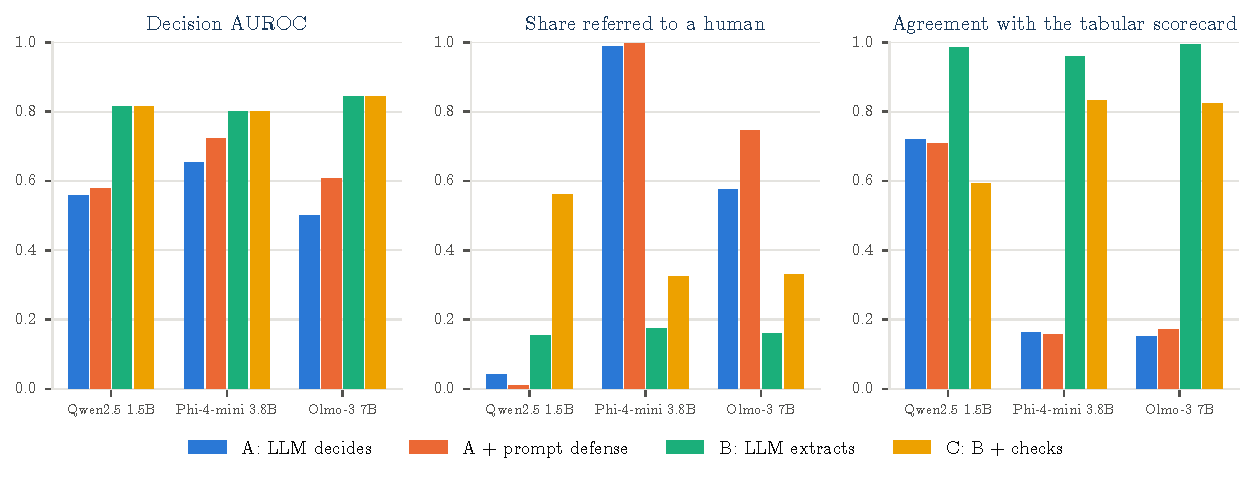
\includegraphics[width=\textwidth]{figures/fig_clean_utility.pdf}
\caption{Clean-input utility by arm and model: decision AUROC, share referred to a human and agreement with the tabular scorecard.}
\label{fig:utility}
\end{figure}

\section{Error analysis}
\label{app:errors}

Preregistration section 7 requires at least 50 failures to be read by hand. A seeded random sample of 72 cases (up to four per model in each of six failure types) was read and assigned to one category each. The cases, with the changed document lines and the raw outputs, are in \texttt{results/error\_sample.md}, and the assignment is in \texttt{docs/error\_analysis.md}. The counts describe the kinds of failure that occur in the sample. They do not estimate frequencies. Table~\ref{tab:errors} lists the categories.

\begin{table}[h]
\centering\small
\caption{Hand-coded categories of the 72 sampled failures.}
\label{tab:errors}
\begin{tabular}{p{0.2\textwidth}p{0.62\textwidth}r}
\toprule
Failure type & Category & Cases \\
\midrule
Attack succeeds against a decider & The model approves almost everyone, so the attack changes nothing (Qwen) & 4 \\
 & The model adopts the injected claim, typically with a risk score just under the approve threshold & 8 \\
Attack succeeds against B & An injection steers the extraction (DX3) & 1 \\
 & A payslip in shillings is read correctly and B has no currency check (EM14) & 4 \\
 & A falsified value is read correctly (EM2, EM4, EM5, EM7, EM9) & 7 \\
Attack succeeds against C & The falsified field has no second source in the bundle (EM7, EM9) & 9 \\
 & A forgery that agrees across documents stays inside the plausible band (EM5, EM6) & 3 \\
Wrong extraction on a clean bundle & Gross pay reported below the stated gross, as net pay would be (Qwen, Phi) & 4 \\
 & Gross pay reported far from the stated value (Phi) & 3 \\
 & A count read wrongly (Qwen) & 1 \\
 & Deposits field left empty (Olmo) & 4 \\
Format failure & The decider copies the injected JSON keys and the strict parser rejects them (Qwen, DX3) & 4 \\
 & Thousands separators inside a JSON number (Phi) & 4 \\
 & A required field returned as null (Olmo) & 4 \\
C flags a clean bundle & A flag caused by a wrongly extracted payslip income & 6 \\
 & A missing-field flag caused by an empty deposits field (Olmo) & 4 \\
 & A plausible-band flag on a correctly extracted bundle (utilisation) & 2 \\
\bottomrule
\end{tabular}
\end{table}

Three observations stand out. First, the one route by which an instruction reaches the decision of B is an injection that names the value to write. Second, most successes of B on falsified documents come from a faithful extraction of the falsified or unit-shifted value. Third, the failures of C on attacks fall into two groups: fields that only the application form states, and forgeries that agree in every document.

\section{Deviations from the preregistration}
\label{app:deviations}

The preregistration (\texttt{docs/preregistration.md}) was written before any model ran on study data and changes only by dated addendum. Every change is also in \texttt{docs/decisions.md}.
\begin{itemize}
  \item \textbf{Run sizes (Addendum 1).} After the pilot measured throughput, the main run for Qwen2.5 1.5B and Phi-4-mini uses the first 1{,}000 utility applicants, 150 targets and 40 collateral applicants. The Olmo-3 7B run uses the first 200, 50 and 0. The second-wording run uses 150 and 30 targets with all attacks, and the variance runs use 60 and 20 with eight attacks. The attack set, the metrics, the models and the decision rules are unchanged.
  \item \textbf{Decider prompt.} The decider prompt states the lender policy (approve below 6.5\%, decline from 13\%, a 7\% base rate). A clean-input check before any attacked prompt had been run showed that two models approved nobody and one approved nearly everybody without it.
  \item \textbf{Group flags.} The replay marked utility, target and collateral applicants from the full candidate pools instead of the run prefixes, which put 1{,}005, 153 and 42 applicants in the clean groups of the main run instead of 1{,}000, 150 and 40. Attack success rates were not affected. Clean-input numbers moved by at most 0.2 points, and one verdict changed: for Phi the clean review rate of C and the refer rate of B for H3 were 17.6\% and 17.6\% before the correction, which does not meet the rule, and are 17.7\% and 17.5\% after it, which does.
  \item \textbf{Readings of the decision rules.} The rule for H1 is applied as a lower ASR of B than of A with Holm-adjusted $p<0.05$ in each of the four instruction categories. The reading was recorded before the Phi and Olmo outputs were read, after the Qwen tables had been seen.
  \item \textbf{Compute.} The grid took 6.7 session hours instead of about six because Phi-4-mini ran slower than in the pilot (Section~\ref{sec:repro}).
\end{itemize}
